\documentclass{article}

\usepackage[english]{babel}
\usepackage[a4paper,top=2cm,bottom=2cm,left=3cm,right=3cm]{geometry}

\usepackage{amsmath}
\usepackage{graphicx}
\usepackage{booktabs}
\usepackage{float}
\usepackage{hyperref}
\usepackage{listings}
\usepackage{microtype}
\usepackage{needspace}
\usepackage{subcaption}
\usepackage{tabularx}

\hypersetup{colorlinks=true, linkcolor=blue, citecolor=blue, urlcolor=blue}

\lstdefinestyle{code}{
  language=C,
  basicstyle=\ttfamily\footnotesize,
  columns=fullflexible,
  keepspaces=true,
  showstringspaces=false,
  frame=single,
  framerule=0.3pt,
  breaklines=true,
  xleftmargin=0.6em,
  framexleftmargin=0.6em,
  aboveskip=0.8em,
  belowskip=0.6em,
  captionpos=t
}

\newcommand{\snippetspace}{\Needspace{16\baselineskip}}

\title{High-Performance Computing\\
       \large MPhil Data Intensive Science}
\author{Barbara Koch \\ University of Cambridge}
\date{\today}

\begin{document}

\maketitle
\begin{abstract}
This coursework develops an in-place Cholesky factorization routine
\(C = LL^T\) in C for a single 76-core CSD3 icelake node, using OpenMP for
shared-memory parallelism.

The implementation was built in stages. I began from the provided baseline
algorithm (\texttt{v1}), then first improved single-thread performance through
better memory access and compiler optimisation (\texttt{v2}). I next added a
straightforward OpenMP parallelisation of the trailing update (\texttt{v3}).
This improved performance at moderate thread counts, but the flat OpenMP
version still synchronised once per column step.

To reduce this overhead, I rewrote the algorithm in blocked form
(\texttt{v4}), processing panels of width \(\mathrm{NB}=96\). This changed the
synchronisation frequency from \(O(n)\) to \(O(n/\mathrm{NB})\) per
factorisation, and strong scaling improved in the measurements. I then introduced
several locality- and throughput-oriented
optimisations in the final version (\texttt{v5}), including column packing,
private per-thread panel storage, four-way unrolling of the trailing update,
and round-robin scheduling in the trailing update phase.

Correctness was checked throughout using exact small examples, reconstruction
residuals, output-layout checks, and agreement across thread counts. Relative
to the \texttt{-O0} baseline, the serially optimised version improves
single-thread performance by around 13--17\(\times\). The blocked OpenMP
version \texttt{v4\_openmp\_blocked} reaches 147.2~GFLOP/s at 76 threads for
\(n=8000\), corresponding to a speedup of 59.5\(\times\) and a parallel
efficiency of 78.2\%. The final implementation,
\texttt{v5\_openmp\_blocked} (tag \texttt{v0.5-tuned}), reaches
182.7~GFLOP/s at 76 threads for \(n=8000\), a 24\% improvement over
\texttt{v4\_openmp\_blocked} at the same thread count.
\end{abstract}

\section{Introduction}

Cholesky factorization is a standard tool in scientific computing whenever a
symmetric positive-definite matrix must be inverted, solved against, or used to
compute a determinant. In the context of covariance matrices, this is
particularly important because the log-determinant can be recovered directly
from the diagonal of the Cholesky factor,
\begin{equation}
  \log |C| = 2 \sum_{p=0}^{n-1} \log L_{pp}.
\end{equation}

For dense \(n \times n\) matrices, the cost of Cholesky factorization is
\(O(n^3)\), so even moderate increases in efficiency can have a large effect on
runtime. The main challenge in this coursework was therefore not only to
produce a correct implementation, but to improve its performance in a controlled
way and to justify each optimisation with measurements.

I approached the coursework as a sequence of implementation stages. First, I
established a working baseline that follows the provided algorithm directly.
Second, I improved its single-thread behaviour by changing loop order and
reducing unnecessary memory traffic. Third, I parallelised the trailing update
with OpenMP and measured how far this simple approach would scale. Finally,
after observing that the flat OpenMP version scaled poorly at high thread
counts, I restructured the algorithm into a blocked form and then optimised the
blocked kernel further for cache locality, instruction-level parallelism, and
load balance.

This report follows that development path. Rather than presenting only the
final code, it explains what was changed at each stage, why the change was made,
and how the measured results motivated the next step. The final implementation,
\texttt{v5\_openmp\_blocked} (tag \texttt{v0.5-tuned}), achieves
182.7~GFLOP/s at 76 threads for \(n=8000\) on a single CSD3 icelake node.

In the reported data, throughput is higher at smaller problem sizes
(for example 238.4~GFLOP/s at \(n=2000\), 76 threads) than at
\(n=8000\) (182.7~GFLOP/s, 76 threads).
\section{Algorithm and Interface}

\subsection{Cholesky recurrence}

The factorisation proceeds column by column for \(p = 0, \ldots, n-1\).
At step \(p\), after the contributions from columns \(0,\ldots,p-1\) have
already been subtracted from the working matrix, the diagonal entry is
\begin{equation}
  L_{pp} = \sqrt{C_{pp}^{(p)}},
\end{equation}
and the entries below the diagonal are
\begin{equation}
  L_{ip} = \frac{C_{ip}^{(p)}}{L_{pp}}, \qquad i > p.
\end{equation}
The remaining trailing submatrix is then updated by
\begin{equation}
  C_{ij}^{(p+1)} = C_{ij}^{(p)} - L_{ip}L_{jp}, \qquad i,j > p.
\end{equation}

\subsection{Function interface}

The function
\begin{verbatim}
double mphil_dis_cholesky(double *c, int n);
\end{verbatim}
takes a pointer to a row-major $n \times n$ matrix and performs the
factorisation in place.

On return:
\begin{itemize}
  \item the lower triangle contains $L$,
  \item the upper triangle contains $L^T$.
\end{itemize}

The function returns the wall-clock time in seconds. Inputs with
$n < 1$ or $n > 100000$ are rejected.

The repository contains five main implementation versions of the routine,
corresponding to successive optimisation stages. These stages are tracked
with tags \texttt{v0.1-baseline} through \texttt{v0.5-tuned}.
The implementation used for the main results is
\texttt{cholesky\_v5\_openmp\_blocked.c} (tag \texttt{v0.5-tuned});
the earlier tagged versions are retained as intermediate development
stages.

\subsection{Correctness verification}

Correctness was assessed using several complementary checks.
The main criterion is the reconstruction error of the factorisation,
rather than the log-determinant alone.

The test suite was run on a CSD3 icelake node for both:
\begin{itemize}
  \item a \textbf{strict build} (without \texttt{-ffast-math}),
  \item a \textbf{performance build} (with \texttt{-ffast-math}),
\end{itemize}
and across multiple thread counts ($T = 1, 2, 4, 8, 76$).
All tests passed in all configurations.

\begin{enumerate}
  \item \textbf{Known-$L$ tests.}
  Matrices of the form $C = L_{\mathrm{ref}} L_{\mathrm{ref}}^T$ were generated,
  and the computed factor was compared directly to $L_{\mathrm{ref}}$.
  Test sizes included values around block boundaries
  ($n = 95, 96, 97$, etc.), where indexing errors are more likely.

  The maximum observed errors were small and consistent with double
  precision accuracy.

  \item \textbf{Output layout.}
  The symmetry between the lower and upper triangles was checked in the test
  suite.

  \item \textbf{Boundary cases.}
  The implementation correctly handles $n=1$ and rejects invalid sizes.

  \item \textbf{Thread consistency.}
  Results obtained with multiple threads were compared to the single-thread
  result. The maximum observed differences were within tolerance
  ($\max|\Delta| < 10^{-10}$).
\end{enumerate}

The log-determinant was used as a secondary check only. While it provides a
useful scalar summary, it does not detect all possible errors (for example,
incorrect off-diagonal entries).

% ======================================================================
\section{Optimisation Strategy}

\subsection{v1 --- Baseline (tag \texttt{v0.1-baseline})}

The baseline implementation follows the provided algorithm and is compiled
with \texttt{-O0}. The trailing update uses a loop ordering where
\texttt{c[i*n+j]} is accessed with a large stride in the inner loop.
For large $n$, this is expected to limit cache efficiency.

\snippetspace
Snippet~\ref{lst:v1} shows the baseline trailing update. Because the matrix is
stored in row-major order, the inner loop over $i$ walks memory with stride
$n$, which gives poor spatial locality.

\begin{lstlisting}[style=code,caption={Baseline trailing-update kernel in v1.},label={lst:v1}]
for (int j = p + 1; j < n; j++) {
    for (int i = p + 1; i < n; i++) {
        c[i*n + j] -= c[i*n + p] * c[p*n + j];
    }
}
\end{lstlisting}

\subsection{v2 --- Serial optimisation (tag \texttt{v0.2-serial-opt})}

Two simple changes are made to improve single-thread performance:

\begin{itemize}
  \item \textbf{Loop interchange.}
  The inner loop is changed to iterate over $j$, making
  \texttt{c[i*n+j]} contiguous in memory. This is intended to improve
  cache locality and may allow the compiler to vectorise the loop more
  effectively.

  \item \textbf{Loop-invariant hoisting.}
  The value \texttt{c[i*n+p]} is reused inside the inner loop, so it is
  loaded once per row instead of once per iteration.
\end{itemize}

\snippetspace
Snippet~\ref{lst:v2} shows the optimised trailing-update kernel. The outer loop
now walks rows, while the inner loop sweeps contiguous elements within each row.

\begin{lstlisting}[style=code,caption={Optimised trailing-update kernel in v2.},label={lst:v2}]
for (int i = p + 1; i < n; i++) {
    double c_ip = c[i*n + p];
    for (int j = p + 1; j < n; j++) {
        c[i*n + j] -= c_ip * c[p*n + j];
    }
}
\end{lstlisting}

With compiler optimisations enabled (\texttt{-O3 -march=native -ffast-math}),
this version is faster than the baseline in the measurements.

\subsection{v3\_openmp --- Flat OpenMP parallelism (tag \texttt{v0.3-openmp-v1})}

The trailing update is parallelised over rows using
\texttt{\#pragma omp for}. Since each row is independent, this is a natural
choice for parallelisation.

A single \texttt{omp parallel} region is used around the outer loop to avoid
repeated thread creation. Within each iteration, \texttt{omp single} is used
for the diagonal and normalisation steps, followed by a barrier before the
parallel update.

\snippetspace
Snippet~\ref{lst:v3} shows the flat OpenMP structure. The key limitation is
that the \texttt{single} and \texttt{for} regions are encountered once per
column, so the algorithm still synchronises at every step.

\begin{lstlisting}[style=code,caption={Flat OpenMP structure in v3.},label={lst:v3}]
#pragma omp parallel default(none) shared(c, n)
{
    for (int p = 0; p < n; p++) {
        #pragma omp single
        { /* diagonal update and normalisation */ }

        #pragma omp for schedule(static)
        for (int i = p + 1; i < n; i++) {
            /* update row i of the trailing submatrix */
        }
    }
}
\end{lstlisting}

This approach improves performance at moderate thread counts. However, for
$n=2000$, performance peaks at around 48 threads and then decreases at higher
thread counts.

\subsection{v4\_openmp\_blocked --- Panel-blocked algorithm (tag \texttt{v0.4-blocked})}

To reduce synchronisation overhead, the algorithm is restructured to process
blocks of columns instead of a single column at a time.

The matrix is processed in panels of width $\mathrm{NB}$. For each panel,
three steps are performed:

\begin{itemize}
  \item \textbf{Phase 1 (serial):} factorise the diagonal block.
  \item \textbf{Phase 2 (parallel):} solve for the block below the panel.
  \item \textbf{Phase 3 (parallel):} update the trailing submatrix.
\end{itemize}

\snippetspace
Snippet~\ref{lst:v4} shows the blocked outer structure. One synchronisation
sequence now covers an entire panel rather than a single column.

\begin{lstlisting}[style=code,caption={Panel-blocked structure in v4.},label={lst:v4}]
#pragma omp parallel default(none) shared(c, n)
{
    for (int k = 0; k < n; k += BLOCK_NB) {
        int kend = (k + BLOCK_NB < n) ? (k + BLOCK_NB) : n;

        #pragma omp single
        { /* Phase 1: factor diagonal block */ }

        #pragma omp for schedule(static)
        for (int i = kend; i < n; i++) {
            /* Phase 2: TRSM below the panel */
        }

        #pragma omp for schedule(guided)
        for (int i = kend; i < n; i++) {
            /* Phase 3: SYRK trailing update */
        }
    }
}
\end{lstlisting}

This reduces the number of global synchronisation points from $O(n)$ to
$O(n/\mathrm{NB})$, which is expected to improve scalability.

The panel width was chosen empirically. Values in the range
$\mathrm{NB}=64$--$256$ were tested. In the committed block-sweep results at
$n=8000$, $\mathrm{NB}=256$ is fastest at 8 and 32 threads.
At 76 threads the differences between $\mathrm{NB}$ values are small and
the measurements are noisier. $\mathrm{NB}=96$ is used for
the main scaling runs.

\subsection{v5\_openmp\_blocked --- Further optimisation (tag \texttt{v0.5-tuned})}

Several additional optimisations are introduced on top of v4. These aim to
improve memory access patterns and increase instruction-level parallelism.

\begin{itemize}
  \item \textbf{Column packing (Phase 1).}
  The column used in the panel update is copied into a contiguous buffer.
  This is intended to avoid repeated long-stride accesses.

  \item \textbf{Per-thread packed panel (Phase 2).}
  Each thread copies the current panel block into a private buffer.
  This is intended to reduce repeated access to widely spaced memory
  locations during the triangular solve.

  \item \textbf{Loop unrolling (Phase 3).}
  The inner update loop is unrolled to process multiple columns at once.
  This is intended to increase the amount of independent work available
  to the processor.

  \item \textbf{Scheduling strategy.}
  \texttt{schedule(static,1)} is used in the trailing update to distribute
  work more evenly across threads, as the amount of work per row increases
  with the row index.
\end{itemize}

\snippetspace
Snippet~\ref{lst:v5} illustrates the most performance-critical part of the
final kernel: the trailing update is assigned round-robin across threads and
the inner work is unrolled to accumulate four dot products at once.

\begin{lstlisting}[style=code,caption={Round-robin scheduling and four-way unrolling in v5.},label={lst:v5}]
#pragma omp for schedule(static, 1)
for (int i = kend; i < n; i++) {
    for (j = kend; j <= i - 3; j += 4) {
        double d0 = 0.0, d1 = 0.0, d2 = 0.0, d3 = 0.0;
        #pragma omp simd reduction(+:d0,d1,d2,d3)
        for (int p = 0; p < panel_width; p++) {
            double pi = panel_i[p];
            d0 += pi * pj0[p]; d1 += pi * pj1[p];
            d2 += pi * pj2[p]; d3 += pi * pj3[p];
        }
    }
}
\end{lstlisting}

These changes are associated with higher measured performance, although
their individual contributions are not isolated in this report. The final
version shows higher measured performance than v4 at both 1 and 76 threads.
% ======================================================================

\section{Experimental Setup}

\paragraph{Platform.}
All experiments were run on a single node of the CSD3 icelake partition. Jobs were submitted using SLURM, typically requesting one full node.

\paragraph{Compilation.}
The following compiler settings were used:

\begin{center}
\begin{tabular}{ll}
\toprule
Version & Flags \\
\midrule
v1 & \texttt{-O0 -g} \\
v2 & \texttt{-O3 -march=native -ffast-math} \\
v3--v5 & \texttt{-O3 -march=native -ffast-math -fopenmp} \\
\bottomrule
\end{tabular}
\end{center}

All versions were compiled with \texttt{gcc} (module \texttt{gcc/11}).

\paragraph{Runtime settings.}
OpenMP threads were pinned to cores using
\texttt{OMP\_PROC\_BIND=close} and \texttt{OMP\_PLACES=cores}.
The number of threads $T$ was varied through
\texttt{OMP\_NUM\_THREADS}.

\paragraph{Methodology.}
Matrix sizes $n \in \{2000, 4000, 6000, 8000\}$ were used to cover a range
of problem sizes.

Thread counts $T \in \{1,2,4,8,16,32,48,64,76\}$ were used to study
strong scaling from a single core to the full node.

Each configuration was run three times. In the committed scaling CSV, the
blocked $n=8000$ points were also measured in a second SLURM job, giving six
timing samples for those points. Means and standard deviations are computed
over all available samples. For \texttt{v5\_openmp\_blocked} at $n=8000$,
the two jobs produced noticeably different timings at $T=8$, which is
visible as a larger error bar at that point in the scaling figures.

Performance is reported in GFLOP/s using the leading-order Cholesky cost,
\[
\mathrm{GFLOP/s} = \frac{n^3}{3t \times 10^9},
\]
where $t$ is the measured runtime.
All timings include only the factorisation routine; setup and validation
are excluded.

The benchmark program records the actual OpenMP thread count at runtime,
so reported values reflect the effective number of threads used.

All figures in the report are generated from CSV data in \texttt{results/}
using the provided plotting scripts.

\paragraph{Git tags.}
The development of the code is tracked using tagged commits, corresponding
to the main optimisation stages:

\begin{center}
\small
\begin{tabularx}{\linewidth}{l l X}
\toprule
Tag & File & Description \\
\midrule
\texttt{v0.1-baseline} &
\texttt{cholesky\_v1\_baseline.c} &
Baseline implementation at \texttt{-O0} \\

\texttt{v0.2-serial-opt} &
\texttt{cholesky\_v2\_serial\_opt.c} &
Improved memory access and compiler optimisations \\

\texttt{v0.3-openmp-v1} &
\texttt{cholesky\_v3\_openmp.c} &
First OpenMP version (parallel trailing update) \\

\texttt{v0.4-blocked} &
\texttt{cholesky\_v4\_openmp\_blocked.c} &
Panel-blocked algorithm \\

\texttt{v0.5-tuned} &
\texttt{cholesky\_v5\_openmp\_blocked.c} &
Final version with improved locality and scheduling \\
\bottomrule
\end{tabularx}
\end{center}

Each tag corresponds to a working version of the code and can be inspected
directly in the repository.


\section{Results}

\subsection{Serial optimisation}

Figure~\ref{fig:serial} shows the effect of the serial optimisations.
Version v2 is around 13--17$\times$ faster than v1 across
$n=500$--$2000$.

Both versions follow the similar slope in the log--log time plot
(Figure~\ref{fig:serialtime}).

\begin{figure}[h]
  \centering
  \begin{subfigure}[b]{0.48\textwidth}
    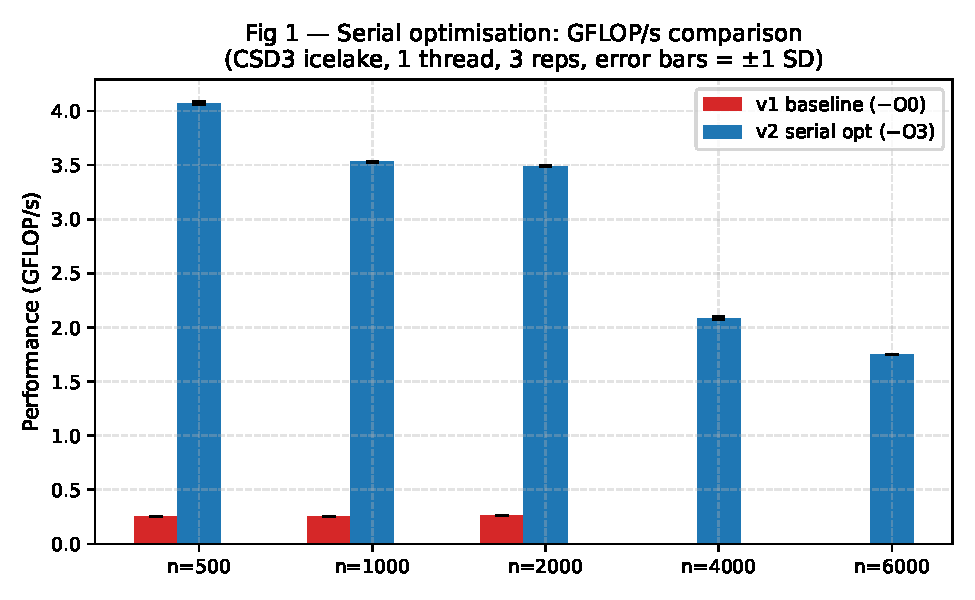
\includegraphics[width=\linewidth]{figures/fig1_serial_gflops.pdf}
    \caption{GFLOP/s for v1 and v2 (1 thread).}
    \label{fig:serial}
  \end{subfigure}\hfill
  \begin{subfigure}[b]{0.48\textwidth}
    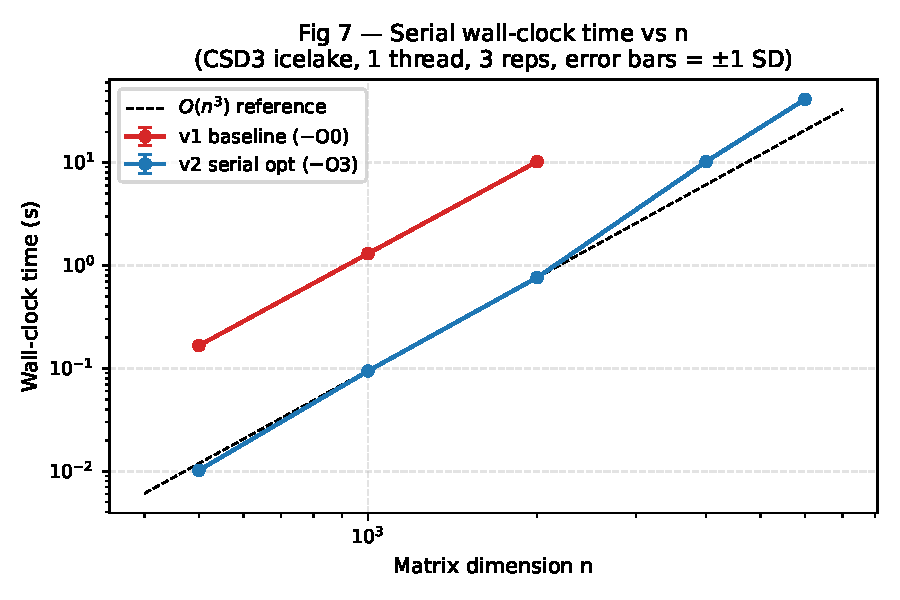
\includegraphics[width=\linewidth]{figures/fig7_serial_time.pdf}
    \caption{Runtime vs.\ $n$ (log--log scale).}
    \label{fig:serialtime}
  \end{subfigure}
  \caption{Serial performance on CSD3 icelake. Mean $\pm$1 SD over 3 runs.}
\end{figure}

\subsection{Incremental optimisation}

Figure~\ref{fig:incremental} shows single-thread performance at each stage.

The transition from v1 to v2 gives the largest improvement.
The v2 and v3 results are similar at 1 thread.
The v5 result is higher than the v4 result at 1 thread.

\begin{figure}[h]
  \centering
  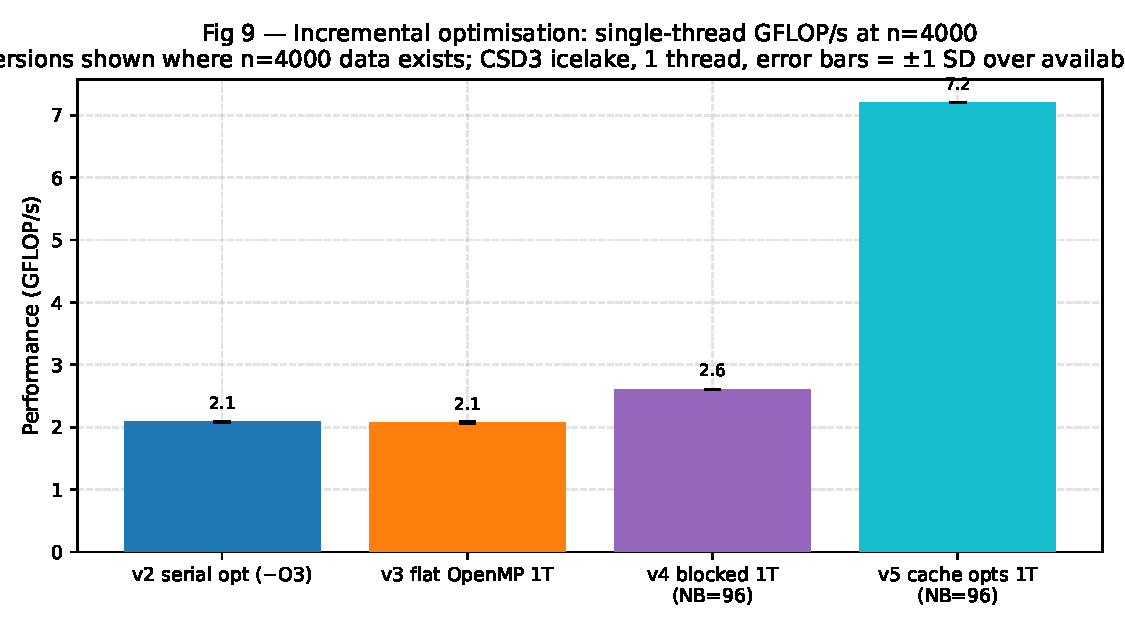
\includegraphics[width=0.7\textwidth]{figures/fig9_incremental.pdf}
  \caption{Single-thread GFLOP/s at $n=4000$ for v2--v5.}
  \label{fig:incremental}
\end{figure}

\subsection{Panel-width selection}

Figure~\ref{fig:blocksweep} shows the effect of panel width for
\texttt{v5\_openmp\_blocked} at $n=8000$.

The best measured panel width depends on thread count in the committed sweep.
NB=256 is fastest at 8 and 32 threads. At 76 threads the differences between
NB values are small and the measurements are noisier. NB=96 is used in the
remainder of the study.

\begin{figure}[h]
  \centering
  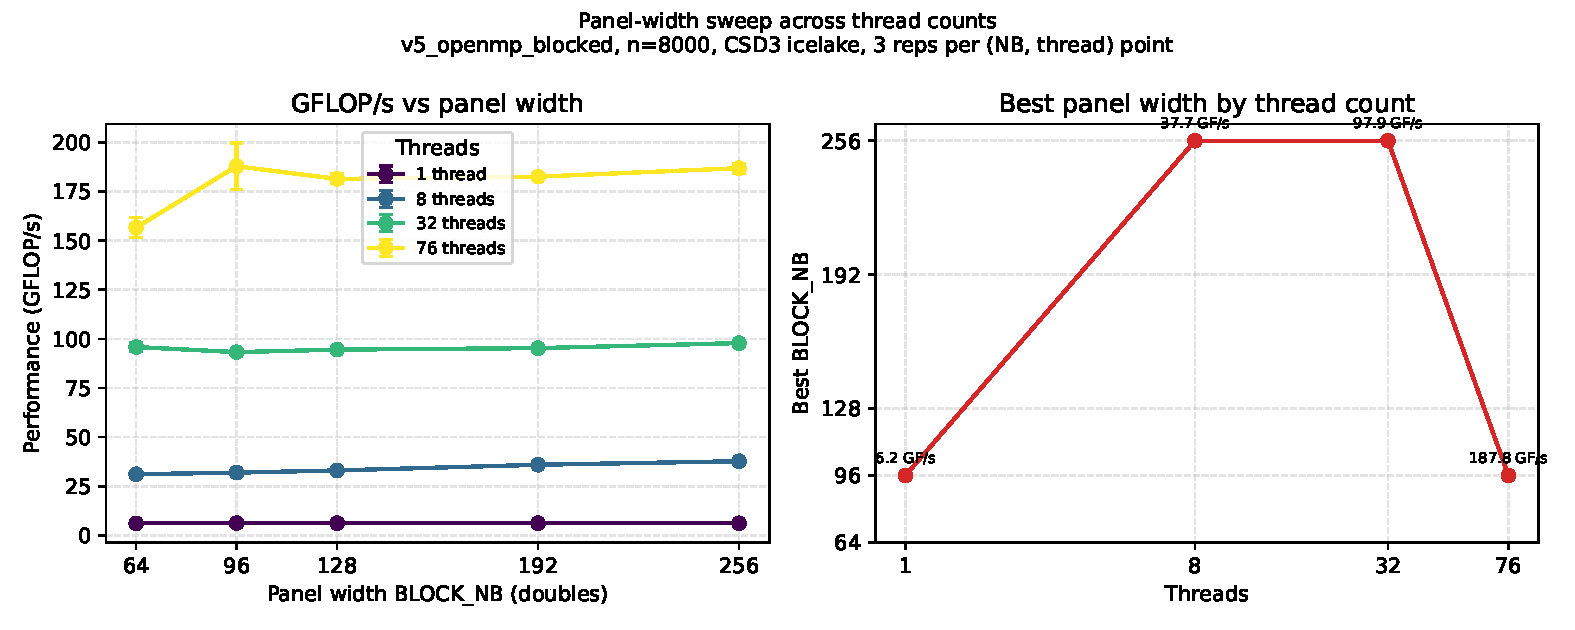
\includegraphics[width=\textwidth]{figures/fig8_block_sweep.pdf}
  \caption{Panel-width sweep for \texttt{v5\_openmp\_blocked} at $n=8000$.}
  \label{fig:blocksweep}
\end{figure}

\subsection{Strong scaling}

Figures~\ref{fig:scaling}--\ref{fig:efficiency} show strong scaling for v3,
v4, and v5.

The v3 implementation improves with thread count initially, but does not
scale well to the full node. At high thread counts the marginal gains
become small.

In contrast, both blocked versions (v4 and v5) scale more consistently.
For $n=8000$, v4 reaches 147.2~GFLOP/s at 76 threads, while v5 reaches
182.7~GFLOP/s.

\begin{figure}[h]
  \centering
  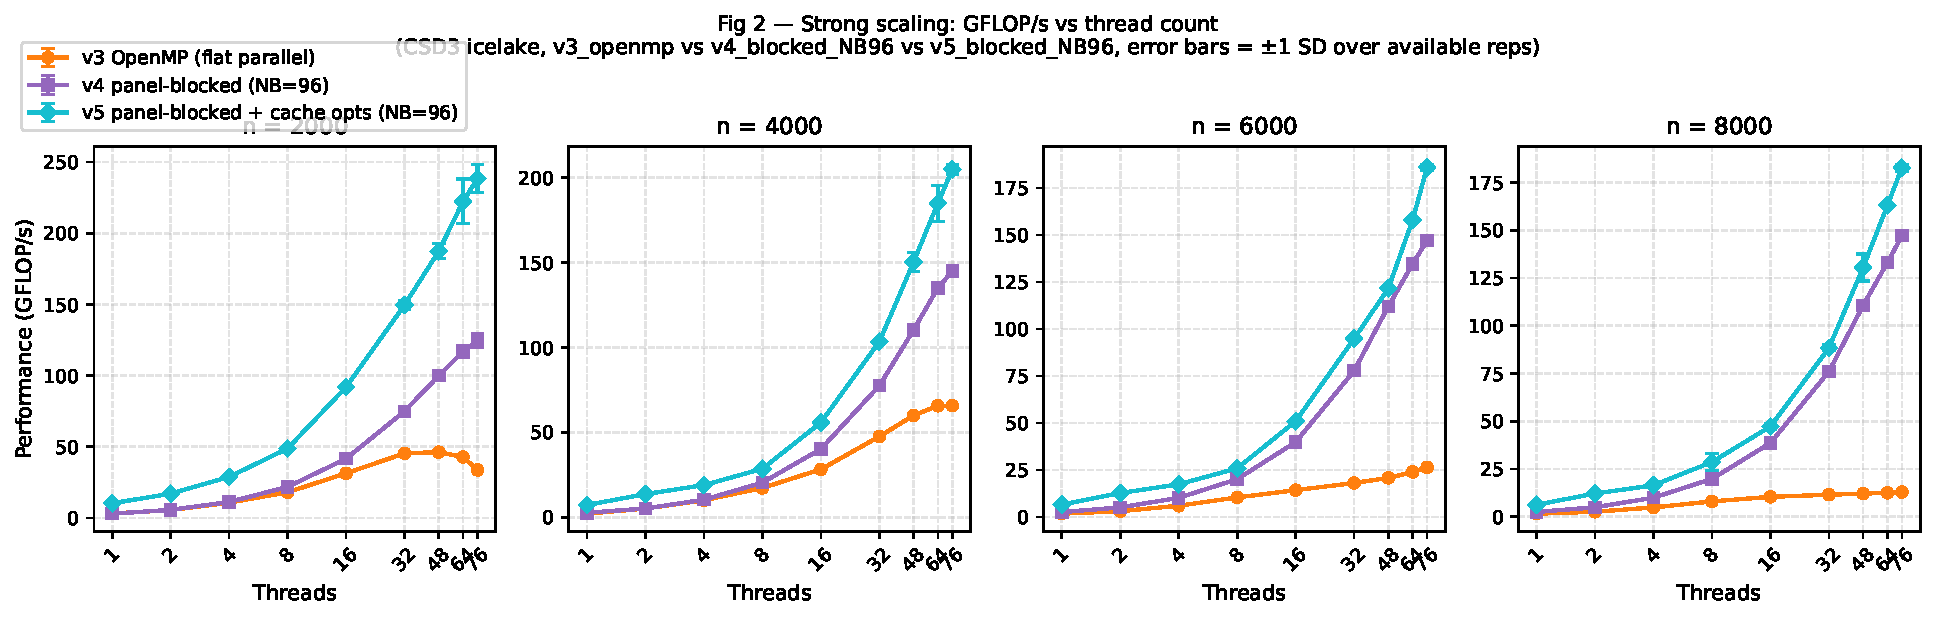
\includegraphics[width=\textwidth]{figures/fig2_scaling_gflops.pdf}
  \caption{GFLOP/s vs.\ thread count for v3, v4, and v5.}
  \label{fig:scaling}
\end{figure}

\begin{figure}[h]
  \centering
  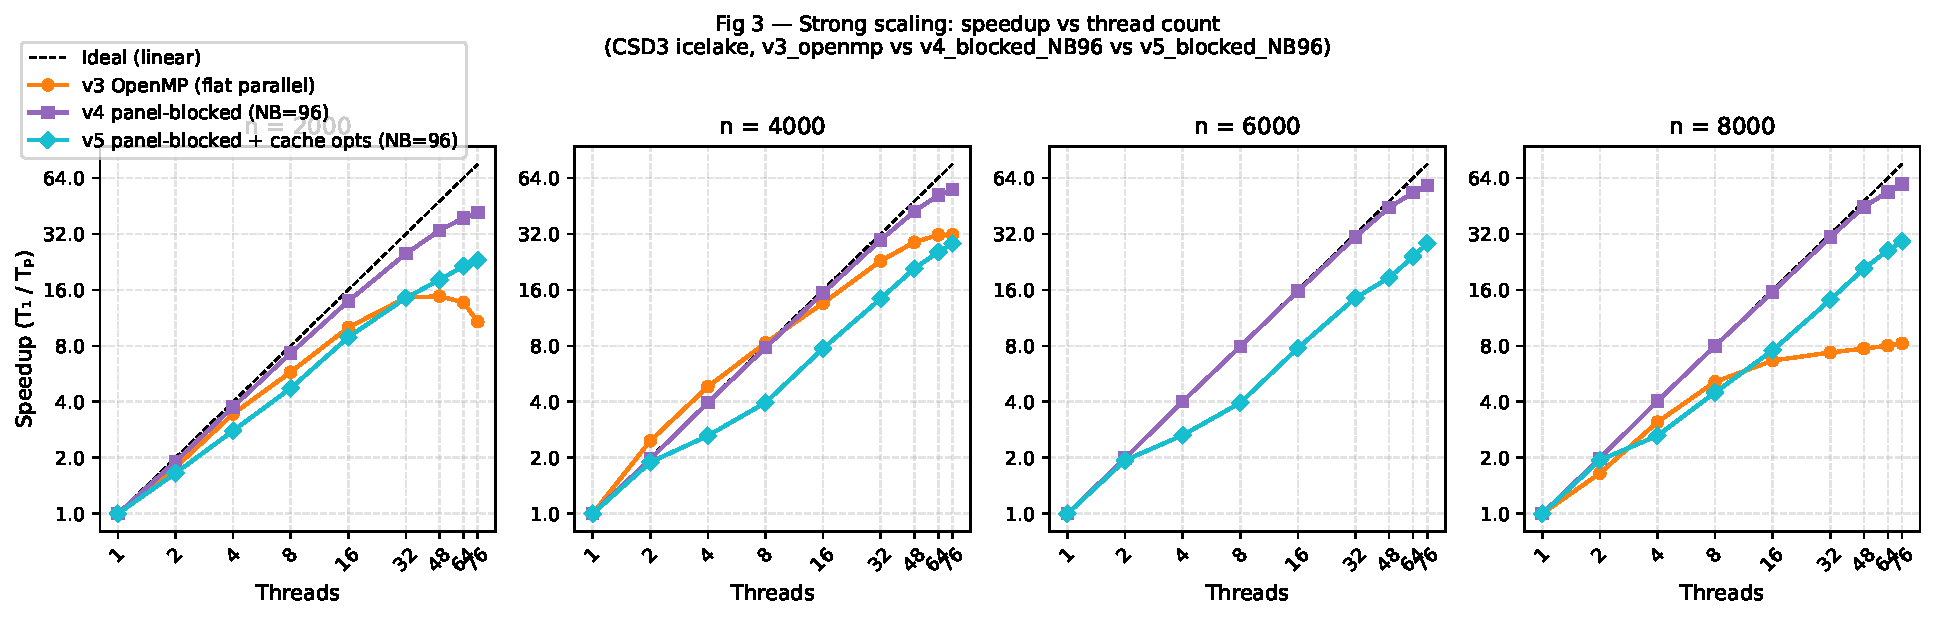
\includegraphics[width=\textwidth]{figures/fig3_scaling_speedup.pdf}
  \caption{Speedup relative to 1 thread.}
  \label{fig:speedup}
\end{figure}

\begin{figure}[h]
  \centering
  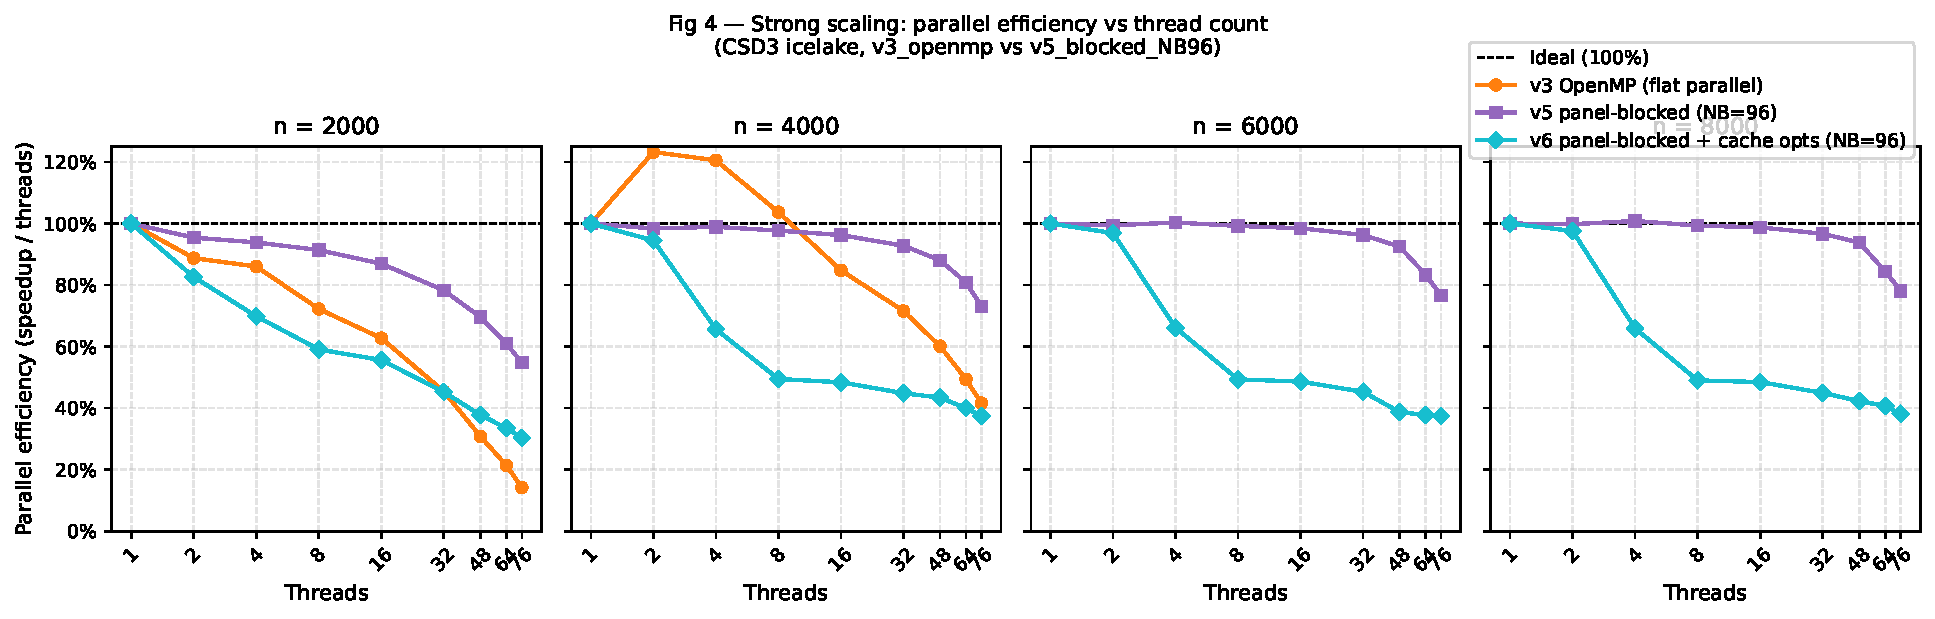
\includegraphics[width=\textwidth]{figures/fig4_scaling_efficiency.pdf}
  \caption{Parallel efficiency vs.\ thread count.}
  \label{fig:efficiency}
\end{figure}

\subsection{Summary at $n=8000$, 76 threads}

\begin{table}[h]
\centering
\caption{Performance at $n=8000$, 76 threads.}
\label{tab:summary}
\begin{tabular}{lrrr}
\toprule
Version & GFLOP/s & Speedup & Efficiency \\
\midrule
v3\_openmp          &  12.9  & 8.2$\times$  & 10.8\% \\
v4\_openmp\_blocked & 147.2  & 59.5$\times$ & 78.2\% \\
v5\_openmp\_blocked & 182.7  & 29.3$\times$ & 38.5\% \\
\bottomrule
\end{tabular}
\end{table}

At $n=8000$, v3 reaches 12.9~GFLOP/s at 76 threads, compared with
147.2~GFLOP/s for v4 and 182.7~GFLOP/s for v5. The lower efficiency of v5
relative to v4 is consistent with its higher 1-thread baseline.

\subsection{Head-to-head comparison}

Figure~\ref{fig:headtohead} compares the three implementations at
$n=8000$.

The difference between the flat and blocked approaches is substantial
in the measurements.
The blocked versions outperform v3 across all measured thread counts.
The improvement from v4 to v5 is smaller but consistent.

\begin{figure}[H]
  \centering
  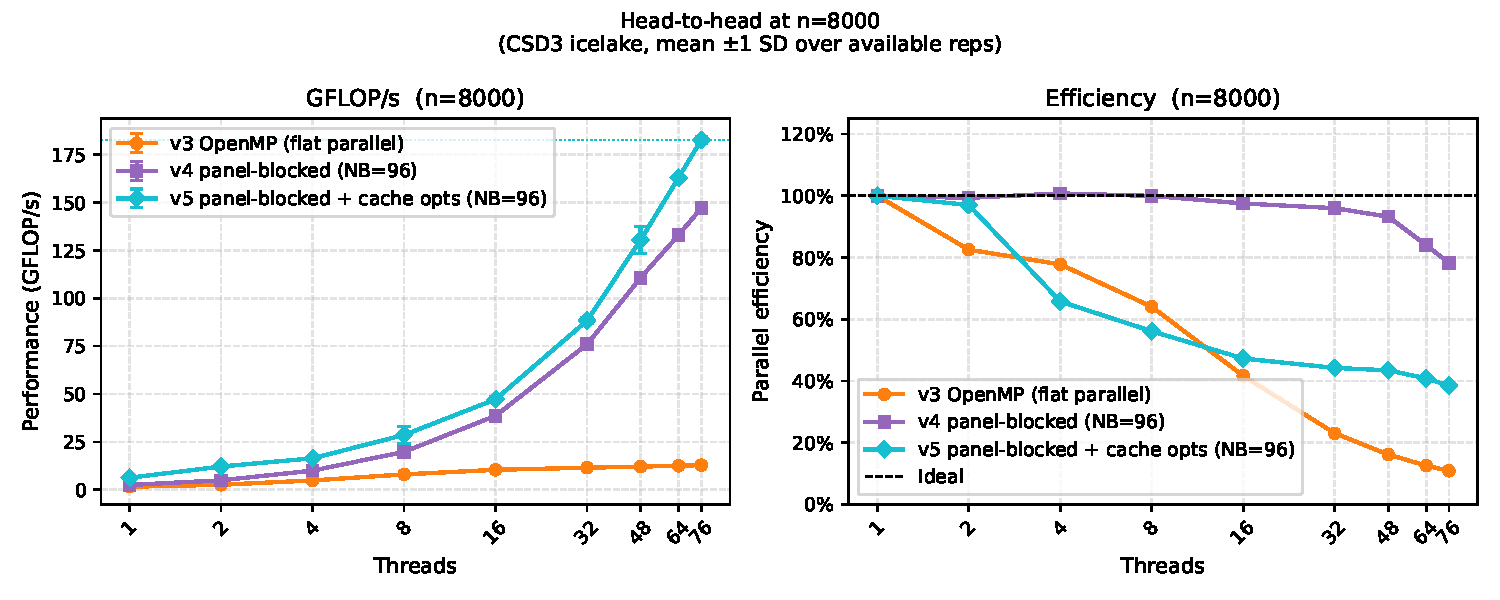
\includegraphics[width=\textwidth]{figures/fig6_v3_v4_v5_n8000.pdf}
  \caption{Comparison of v3, v4, and v5 at $n=8000$.}
  \label{fig:headtohead}
\end{figure}

\subsection{Problem-size scaling}

Figure~\ref{fig:problemsize} shows performance of v5 as a function of $n$.

Performance is highest at smaller sizes and decreases as $n$ increases.
This trend is consistent across most thread counts.

At 76 threads, performance decreases from 238.4~GFLOP/s at $n=2000$
to 182.7~GFLOP/s at $n=8000$.

\begin{figure}[H]
  \centering
  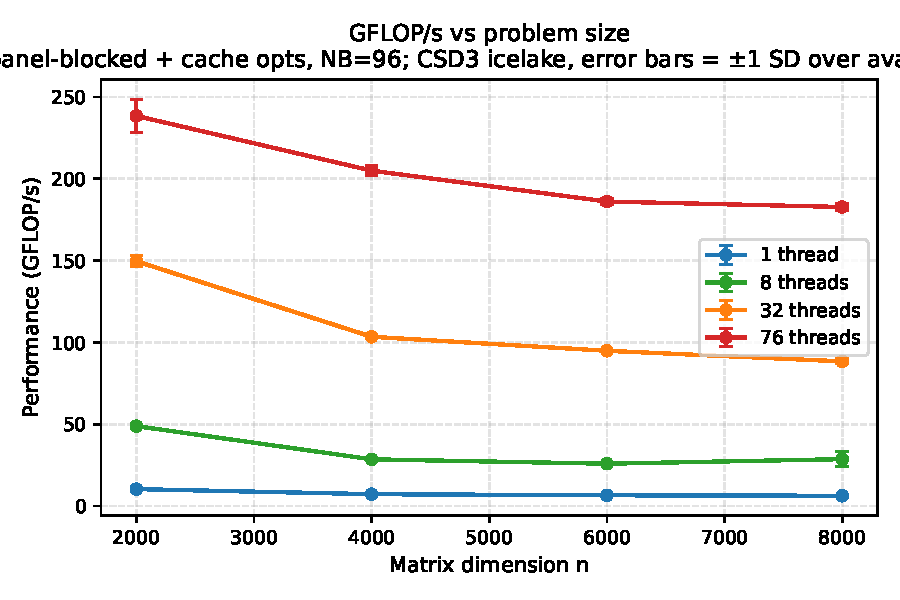
\includegraphics[width=0.62\textwidth]{figures/fig5_problem_size.pdf}
  \caption{GFLOP/s vs.\ problem size for v5.}
  \label{fig:problemsize}
\end{figure}

\section{Discussion}

\paragraph{Scaling behaviour.}
The committed performance data shows three main patterns. First, the flat
OpenMP version improves over its 1-thread baseline but remains well below the
blocked versions at high thread counts. Second, the blocked versions extend
scaling further, with \texttt{v5\_openmp\_blocked} giving the highest reported
performance in the main $n=8000$ comparison. Third, for
\texttt{v5\_openmp\_blocked}, the reported GFLOP/s at 76 threads decreases as
$n$ increases from 2000 to 8000.
% ======================================================================
\section{Conclusion}

Starting from a simple baseline implementation, a series of
optimisations were applied to improve both single-thread and
multi-thread performance.

Basic compiler optimisations and loop restructuring provided a large
improvement on a single core.
Introducing OpenMP parallelism gave further gains, although scaling
was more limited in the flat version than in the blocked versions in the
reported runs.

Rewriting the algorithm in a blocked form improved scalability by
reducing the number of synchronisation points.
Additional changes aimed at improving data locality and loop structure
further increased performance.

The final implementation (\texttt{v5\_openmp\_blocked}) reaches
182.7~GFLOP/s at 76 threads for $n=8000$ on a CSD3 icelake node.
\end{document}
